\chapter{Zaplecze technologiczne - wykorzystane biblioteki}
\label{chapter:libs}

\section{Wybór narzędzi do pracy}
	Złożoność aplikacji, opisana w rozdziale \ref{chapter:app_functional_requirements}, wymagała narzędzi potrzebnych do sprostania poszczególnym wymogom funkcjonalnym. Z prostej przyczyny opcja wielu zewnętrznych bibliotek została odrzucona: zbyt wielka ich ilość z czasem mogłaby stać się problemem, z uwagi na ewentualne konflikty między nimi lub wzrost liczby zależności przechodnich. 
	
	W pierwszej kolejności wybrany został szkielet aplikacji, który w założeniu stanowić miał solidny fundament, na którym oparta została by aplikacja. Spośród wielu dostępnych rozwiązań zdecydowano się, w pierwszej kolejności, na wybór tych, które wspierają \textbf{Dependency Injection} oraz \textbf{Inversion Of Control}. Obie techniki pozwalają znacząco podnieść jakość kodu, zminimalizować stopień kohezji oraz zależności między klasami. Jest to możliwe, ponieważ odpowiedzialność za sterowanie przepływem programu zostaje przeniesiona na szkielet, co odciąża programistę od konieczności kontrolowania tych aspektów. 
	
	Po analizie rozwiązań takich jak \textbf{JBoss Seam Framework}, \textbf{Google Guice}, \textbf{PicoContainer} i \textbf{Spring Framework}, okazało się, że wszystkie z nich wspierają wymienione techniki. Niemniej stopień w jakim można by użyć jednego z nich do kompleksowego wsparcia aplikacji praktycznej nie był już jednakowy. Zaczynając od \textbf{PicoContainer} oferującego wsparcia jedynie dla \textbf{Dependency Injection}, a kończąc na \textbf{Spring Framework} oraz \textbf{JBoss Seam Framework} posiadających najbogatszy wachlarz możliwości, najlepszym wyborem okazuje się być \textbf{Spring}. Z uwagi na popularność w środowisku programistów, stanowi on doskonały kompromis między tym, co oferuje, a tym czego wymaga. Dzięki przyjętemu, przez szkielet, modelowi programistycznemu, opierającemu się o wykorzystanie interfejsów, zamiast konkretnych ich implementacji, \textbf{Spring} jest rozwiązaniem wysoce konfigurowalnym. Nic nie stoi na przeszkodzie, aby do gotowej aplikacji dołączyć dowolną zewnętrzną bibliotekę, czy też zmienić sposób, w jaki dany moduł działa, poprzez dostarczenie własnej implementacji pewnego algorytmu. 
	
\clearpage
\section{Słownik pojęć} 			Poniższa tabela przedstawia definicję pojęć technicznych wykorzystanych w pracy dyplomowej. 
\begin{center}
	\begin{longtable}{| p{3cm} | p{13cm} |}
		\caption[Adnotacje Spring opisujące poziom abstrakcji cache]{
			Adnotacje Spring opisujące poziom abstrakcji cache				
		}\tabularnewline	
		
		\hline
			\multicolumn{1}{|c|}{\textbf{Pojęcie}} 		&
			\multicolumn{1}{|c|}{\textbf{Znaczenie}} 		\\
		\hline
		\endfirsthead
		
		\multicolumn{2}{c}
		{{\bfseries \tablename\ \thetable{} -- kontynuacja...}} \\
		\hline
			\multicolumn{1}{|c|}{\textbf{Pojęcie}} 		&
			\multicolumn{1}{|c|}{\textbf{Znaczenie}} 		\\
		\hline
		\endhead
			
		\hline
			\multicolumn{2}{|r|}{{Następna strona...}} 	\\
		\hline
		\endfoot

		\hline
		\endlastfoot	
		% body of the table
		\textbf{Dependency injection}							&
		\label{concept:di}
		Wstrzykiwanie zależności - jest to technika programistyczna, w której dana klasa nie jest odpowiedzialna za tworzenie obiektów od których zależy.
		Zależność jest umieszczana w danym obiekcie, po jego utworzeniu, przez specjalnego zarządcę, posiadającego wiedzę o wszystkich obiektach istniejących w działającej aplikacji.
		Pozwala to jednocześnie na obniżenie ścisłej zależności między dwoma klasami, a także zmniejsza zapotrzebowania na zasoby systemowe. Jest to możliwe, ponieważ, bardzo często,
		obiekty, będące zależnościami dla innych, istnieją w kontekście danego programu, jako \textbf{singletony}. 
		\hline
		\textbf{Singleton}										&
		\textbf{Singleton} jest wzorcem programistycznym, zakładającym istnienie tylko jednego obiektu danej klasy w całej aplikacji. Najczęściej taka funkcjonalność, realizowana jest poprzez
		utworzenie klasy, która nie posiada publicznego konstruktora, a jej obiekt uzyskiwany jest poprzez statyczną metodę, zwracającą obiekt tej klasy. W kontekście szkieletów aplikacji, wspierających
		\textbf{wstrzykiwanie zależności}, wzorzec singletonu realizowany jest na poziomie zarządcy.
		\hline
		\textbf{Zależność przechodnia}							&
		\label{concept:indirect_dependency}
		Taka zależność pojawia się w momencie kiedy aplikacja korzysta z biblioteki, która z kolei
		korzysta z innych. Skutkiem tego jest, że aplikacja staje się zależna od bibliotek od których 
		bezpośrednio nie zależy. Staje się to problematyczne, w momencie kiedy programista
		zaczyna wykorzystywać funkcjonalność zdefiniowaną w nich, nie wiedząc o tym. Usunięcie bezpośredniej zależności,
		skutkować będzie błędami kompilacji.
		\hline
		\textbf{Obiekt domenowy}								&
		\label{concept:domain_object}
		Klasy takich obiektów zdefiniowane są w modelu danych. 
		Innymi słowy dostarczają one informacji opisujących, w sposób abstrakcyjny, 
		rzeczywiste obiekty wykorzystywane w aplikacji.	
		\hline
		\textbf{Repozytorium}									&
		\label{concept:repository}
		Abstrakcyjne pojęcie odnoszące się do klasy obiektów - interfejsów leżących na linii
		baza danych - aplikacja, pośredniczących w operacjach zapisu/odczytu. Implementują ideę
		stojącą za pojęciem CRUD.
		\hline
		\textbf{CRUD}
		\label{concept:crud}									&
		Anglojęzyczny skrót wykorzystywany w programowaniu opisujący 4 podstawowe operacje, wykonywany
		na pewnym źródle danych. 
		\begin{itemize}
			\item create - utworzyć,
			\item read - odczytać,
			\item update - uaktualnić, zmodyfikować, 
			\item delete - usunąć
		\end{itemize}	
		\hline
		\textbf{Cache}											&
		\label{concept:cache}
		Cache jest specjalnym obiektem przeznaczonym do czasowego przechowywania danych
		w pamięci dla zapewnienia szybszego dostępu niż w przypadku odwoływania się do 
		bazy danych, plików lub metod wykonujących kosztowne 
		obliczeniowo operacje.
		\tabularnewline
		\hline
		\textbf{ATP}											&
		\label{concept:atp}
		Pojęcie odnosi się do przetwarzania adnotacji języka Java i wykonywania pewnych operacji
		i/lub generowania wyniku.
		\hline
		\textbf{Adnotacje}										&
		\label{concept:annotation}
		Ideą adnotacji jest dodawanie do kodu źródłowego 
		aplikacji metadanych.
		\hline
		\textbf{AOP}											&
		\label{concept:aop}
		\textbf{Aspect Oriented Programming} jest paradygmatem programistycznym zwiększającym
		skalowalność, zmniejszającym kohezję klas i tym samym eliminującym tak zwane \textit{ścisłe zależności}. 
		Programowanie z jego wykorzystaniem odwołuje się do organizacji kodu w tak zwane \textit{aspekty} realizujące
		pewną logikę. Aspekt swoim zasięgiem jest w stanie objęć więcej niż jeden poziom abstrakcji
		zdefiniowany z użyciem technik programowania obiektowego jak na przykład wzorce strategii 
		czy też fabryk.
		\hline 
		\textbf{Kohezja}										&
		\label{concept:cohesion}
		Kohezja, w odniesieniu do programowania, 
		oznacza stopień w jakim dwie klasy są zależne 
		od siebie.
		\hline 
		\textbf{ORM}										&
		\label{concept:orm}
		Z angielskiego, \textbf{Object/Relational Mapping}, jest to technika programistyczna, w założeniu implementująca
		proces konwertowania danych, które nie są obiektami, jak krotki w bazie danych, na model zaprojektowany, zgodnie
		z wytycznymi programowania obiektowego. W wyniku tego, programista uzyskuje dostęp do wirtualnej bazy danych. 
		\hline 
		\textbf{Getter/Setter}									&
		\label{concept:getter_setter}
		Zwyczajowe pojęcia opisujące metody 
		dostępowe klasy służące do pobierania lub ustawienia 
		wartości pól obiektów tej klasy
		\hline
		\textbf{API}											&
		\label{concept:api}
		Ściśle określony zbiór reguł i metod, dzięki którym program może się komunikować ze sobą lub z innym programem.
		\hline
		\textbf{JMS}											&
		\label{concept:jms}
		\textbf{Java Message Service} to część języka Java, która pozwala dwóm i więcej programom komunikować się
		poprzez jednolity interfejs oraz format wiadomości \cite{java_jms}.
		\hline
		\textbf{JMX}											&
		\label{concept:jmx}
		\textbf{Java Management Extensions} jest technologią, która jest częścią standardowej biblioteki Java.
		Dzięki JMX można kontrolować stan aplikacji i urządzeń oraz dynamicznie wpływać na ich stan \cite{java_jmx}.
		\hline	
		\textbf{Best practice}									&
		\label{concept:best_practices}
		Zalecane i pożądane sposoby realizacji często spotykanych problemów, które można napotkać, podczas projektowania
		aplikacji			
		\hline
		\textbf{DRY}
		\label{concept:dry}										&
		\textbf{Dont Repeat Yourself} - zasada negująca implementacje rozwiązań problemów, które już zostały rozwiązane.
		\hline
		\textbf{Artefakt}										&
		\label{concept:artifact}
		Artefakt, w kontekście programowania obiektowego w Java, jest pojęciem jednocześnie opisującym takie elementy tego
		języka jak klasy, interfejsy oraz paczki (zbiór klas i interfejsów).
		\hline
		\textbf{Predykat}										&
		\label{concept:predicate}
		Predykat, coś co umożliwia ustalenie czegoś. Predykat można rozumieć jako kompozycję wyrażań logicznych lub specjalny 
		rodzaj metody weryfikującej zadany problem pod kątem ustalenia wartości prawda/fałsz.
		\hline
		\textbf{Classpath}										&
		\label{concept:classpath}
		\textbf{Classpath} - ścieżka klas, jest parametrem maszyny wirtualnej Java, który wskazuje na lokalizację folderu w systemie plików, gdzie znajduje 
		się skompilowane klasy Javy.
		\hline
		\textbf{Rewizja}										&
		\label{concept:revision}
		Rewizja jest specjalnym numerem, który jest bezpośrednio związany z historią zmian obiektu domenowego. Każda modyfikacja takiego obiektu oznacza w 
		praktyce utworzenie nowej rewizji. 
		\hline
		\textbf{Lokalizacja}									&
		Lokalizacja, w kontekście dowolnej aplikacji, należy rozumieć jako możliwość programu do wsparcia więcej niż jednego języka interfejsu użytkownika.
		\hline
		\textbf{Przypadek użycia}								&
		Sposób opisu wymagań aplikacji na poziomie interakcji między użytkownikiem aplikacji, a nią samą lub konkretna sytuacja występująca w programie.
	\end{longtable}
	\label{app:ehcache:spring_caches}
\end{center}
\section{Szkielet aplikacji}		\subsection{Znaczenie szkieletów aplikacji}
	Internetowe szkielety aplikacji nie są same w sobie bibliotekami programistycznymi. Stanowią one raczej ich zbiór, jak również zestaw narzędzi, mających na celu ułatwienie programiście implementacji własnego rozwiązania. Bardzo często są one również praktyczną implementacją standardów (tak jak \textbf{Seam Framework}) i tak zwanych \textbf{best practices}. Jest to szczególnie użyteczne ponieważ nierzadko zdarza się, że programista popełnia błąd na pewnym etapie projektowanie lub implementacji określonego modułu, którego późniejsze konsekwencje wymagają stworzenia niepotrzebnego i nadmiarowego kodu, czego dałoby by się uniknąć, gdyby podążano już wyznaczonymi ścieżkami. Prawdziwe w takim wypadku staje się również zdanie, że jeden błąd generuje kolejne, a te mogą być zalążkiem następnych.
	
	Powodem istnienia szkieletów aplikacji jest więc zapobieganie takim sytuacjom, poprzez proponowanie już gotowych modułów, które są przetestowane i ciągle modyfikowane przez doświadczone osoby, celem dostarczenia jeszcze lepszych rozwiązań \cite{art_of_java_web_dev}.
	
	Oprogramowanie zorientowane obiektowo jest doskonałym zobrazowaniem koncepcji wykorzystania szkieletu jako fundamentu do budowy własnego rozwiązania. Na najniższym poziomie szczegółowości każdy program czy też moduł większej części, jest zbiorem klas posiadającym jasno określony zbiór ról - obowiązków, a których obiekty współpracują ze sobą, celem dostarczenia gotowego wyniku lub jego części. Wspólnie te obiekty reprezentują pewną koncepcję, dla realizacji której zostały utworzone. 
	
	W kontekście szkieletu aplikacji internetowych można więc wyróżnić klasy przeznaczone do kooperacji z bazą danych, odpowiedzialnych za walidację informacji czy też pomocnych w momencie renderowania widoku. Warto nadmienić, że te zasady są równie ważne dla małych systemów, jak i dla dużych. Niemniej, w pierwszym przypadku, gdzie poziom skomplikowania jest niski, nie ma potrzeby definiowania wielu poziomów abstrakcji ułatwiających określone czynności, jak na przykład wcześniej wymienione walidacje danych. Niestety z czasem, początkowo prosty system, staje się coraz bardziej skomplikowany i bardzo często programista nie jest już wtedy w stanie zapanować na chaosem oraz dostarczyć zunifikowanego sposobu rozwiązywania powtarzalnych czynności. Z tego powodu dobry szkielet programistyczny charakteryzuje się jasno, ale nie sztywno zdefiniowanymi granicami między poszczególnymi zbiorami funkcjonalnymi. Wprowadzone poziomy abstrakcji, często więcej niż jeden dla pojedynczego celu, jak na przykład sposób interakcji systemu i jego klientów, są wynikiem wieloletnich zmian, podczas których zidentyfikowano wiele wspólnych problemów i dla których znaleziono rozwiązanie w postaci ram projektowych czy też \textbf{best pratices}, będących ostatecznie właściwą esencją znaczenia szkieletu aplikacji \cite{framework_design_-_a_role_modeling_approach}.
	
	Dobrymi przykładami tutaj będą z pewnością warstwy abstrakcji dla obsługi operacji bazodanowych. Zawierają one konkretne implementacje, posiadające funkcjonalność odpowiedzialną za wykonanie tych operacji na praktycznie elementarnym poziomie, zostawiając właściwą warstwę logiki w tworzonej aplikacji, odciążają one programistę od przysłowiowego wynajdowania koła od nowa. Praktyczną realizacją tej koncepcji jest na przykład \textbf{Spring Data} pozwalające na napisanie kodu, którego głównymi zaletami będzie odseparowanie logiki biznesowej od wybranej bazy danych oraz wyraźny podział na klasy odpowiedzialne za operacje \textbf{CRUD} na danych, jak i te wykonujące operacje biznesowe. Inne przykłady to między innymi \textbf{EJB}, czy też moduł innego szkieletu programistycznego \textbf{GWT} wykonującego identyczne zadanie. Warto nadmienić, że również warstwy odpowiedzialne za tworzenie i zarządzanie widokiem (warstwa prezentacji) oraz takie, których nadrzędnym celem jest pośredniczenie między widokiem a danymi, są potencjalnymi kandydatami do wyodrębnienia pewnego zbioru funkcjonalności, jako części składowych gotowego szkieletu aplikacji. 
	
\paragraph{Problemy szkieletów aplikacji} \hspace{0pt} \\
	Mimo że szkielety aplikacji znacząco podnoszą jakość kodu oraz obniżają późniejsze koszty jej utrzymania, nie są doskonałym narzędziem. Większość trudności, jakie można napotkać podczas korzystania z nich, wynika z ich rozmiaru oraz ze złożoności. Złożoność należy rozumieć zarówno w kontekście tego, jak dany szkielet jest zaprojektowany, oraz w kontekście wielu obszarów funkcjonalnych, które wspiera. Poniższe zestawienie podsumowuje najczęściej spotykane problemy, z którymi można zetknąć się podczas korzystania ze szkieletów aplikacji:
	\begin{itemize}
		\item \textit{złożoność modelu klas} - obiekty klas zaimplementowane w szkielecie aplikacji współpracują ze sobą, wielokrotnie w więcej niż jednym kontekście. Definiowanie funkcjonalności danej klasy poprzez użycie pojedynczej klasy abstrakcyjnej lub interfejsu jest rozwiązaniem zbyt sztywnym, ponieważ często większa część zdefiniowanych metod nie będzie wykorzystywana w innym miejscu,
		\item \textit{skupienie się na szczególe, pominięcie ogółu} - w momencie projektowania klas, tj. kreowania późniejszego celu istnienia ich obiektów, zdarza się, że gubi się obraz całości zbytnio skupiając się na poszczególnych przypadkach,  \item \textit{złożoność współpracy} - mechanizmy współpracy obiektów odpowiadających, przykładowo za komunikację klient-serwer, mogą stać się zbyt skomplikowane,
		\item \textit{trudnością użycia} - brak drobiazgowej dokumentacji może skutkować użyciem szkieletu w sposób niezamierzony przez jego twórców, co może skutkować implementowaniem kodu, zadaniem którego jest obejście problemu, a nie jego zrozumienie. Nie jest to jedynie aspekt dotyczący samego szkieletu, ale także aplikacji z niego korzystającej. Mimo wszystko nadmiarowy kod wciąż bazuje na klasach danej biblioteki. Zmiany zachodzące w platformie propagują do opartej o nią aplikacji, a działający wcześniej kod, przestaje działać. Programista aplikacji tworzy kolejny, jeszcze bardziej skomplikowany, aby uzyskać funkcjonalność, rzekomo nie dostarczoną przez szkielet programistyczny.
	\end{itemize}
	
	\\
	Rozwiązaniem tych trudności jest zmiana koncepcji, według której projektowany był szkielet aplikacji. Tradycyjne podejście, oparte o klasy, zostaje zastąpione podejściem opartym o role. Idea zakłada wykorzystanie istniejących klas, które grupowane są w bloki funkcjonalne. Każdy z takich bloków to inna rola, a każdy obiekt posiada swoją własną, podrzędną rolę. Dzięki temu szkielet staje się zbiorem funkcji, które z kolei składają się z wielu ról, współpracujących ze sobą dla uzyskania konkretnego wyniku. Tak zaprojektowana i podzielona platforma jest łatwiejsza w zrozumieniu i wykorzystaniu dla celów programów, opartych o nią \cite{framework_design_-_a_role_modeling_approach}.
	
\paragraph{Funkcjonalność szkieletów aplikacji} \hspace{0pt} \\
	Szkielety aplikacji dostarczają jednolitego sposobu budowania programów o nie opartych. Zestawy najlepszych praktyk, komponenty realizujące powtarzalne operacje, a także sposoby realizacji najczęściej spotykanych problemów, to wspólny mianownik szkieletów programistycznych, nie tylko tych przeznaczonych dla aplikacji internetowych. Dla tego typu programów, istniejące rozwiązania, implementują:
	\begin{itemize}
		\item wsparcie dla wielojęzycznych aplikacji,
		\item wsparcie dla różnych rodzajów widoku (strony HTML, strony JSP, pliki PDF lub Excel),
		\item integrację z językiem szablonów pozwalającym, w strukturę strony HTML, dodawać elementy generujące dynamiczne treści,
		\item dostęp do danych oraz ich walidację,
		\item wsparcie dla komunikacji klient - serwer w kontekście mapowania akcji wykonywanych przez użytkownika,
		\item wsparcie dla formularzy internetowych,
		\item wsparcie dla technologii Ajax
	\end{itemize}	
	
\subsection{Spring Framework}
	\textbf{Spring} jest szkieletem tworzenia aplikacji w języku Java dla platformy Java (Standard Edition oraz Enterprise Edition) opisywanym jako \textit{lekki szkielet aplikacji}. Lekkość szablonu odnosi się tutaj nie do rozmiarów całości, ale do filozofii, jaka przyświecała i cały czas przyświeca \textbf{Spring'owi}. Nie wymusza konkretnego stylu programowania czy też używania konkretnych zewnętrznych bibliotek, jednocześnie dając możliwość praktycznie dowolnej integracji. Dobrym przykładem jest mnogość opcji, które można wybrać w przypadku pisania warstwy widoku aplikacji internetowej. Spring oferuje wsparcie czystego JSP (ze wsparciem tagów JSTL) jednocześnie dając możliwość użycia takich bibliotek jak Velocity, FreeMarker, XSLT czy Apache Tiles. Ponadto oparty jest o koncepcję, gdzie poszczególne klasy powiązane są z konkretną rolą, jaką spełniają w programie. Dzięki temu cała platforma jest łatwa w zrozumieniu. Jest to także powód dla którego \textbf{Spring}'a, nie należy rozumieć jako biblioteki, która jednocześnie wspiera więcej niż jeden obszar, ale jako zbioru samodzielnych komponentów. Poprzez wzajemną integrację, każda część szkieletu to rozwiązania innego problemu. Programista może wybrać tę część najlepiej odpowiadającą jego potrzebom.
	\begin{figure}[h]
		\centering
		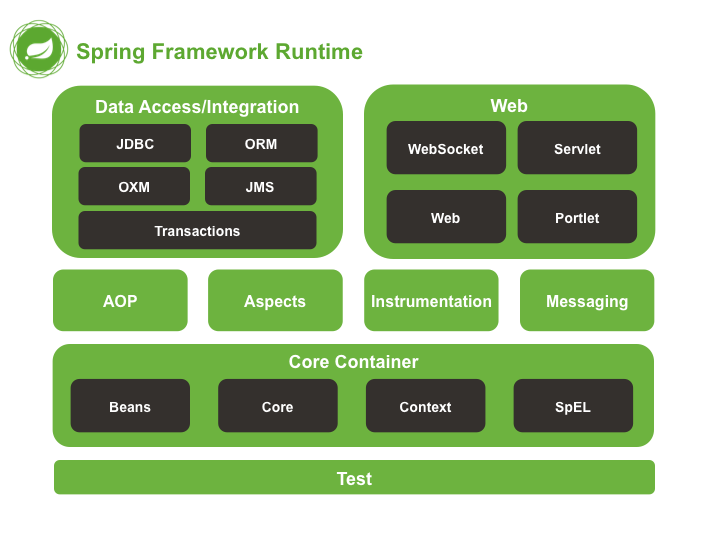
\includegraphics[width=0.95\textwidth]{images/spring-overview}
		\caption[Kontener Spring]{Kontener Spring wraz z modułami\\źródło: \cite{spring_documentation_reference}}
		\label{c3:information_level_figure}
	\end{figure}	
	 \textbf{Spring} składa się z ponad 20 samodzielnych modułów:
	 \begin{itemize}
	 	\item \textbf{Core Container} - fundament szkieletu na którym oparte są pozostałe modułu. Definiuje on funkcjonalność \textbf{Dependency Injection} oraz odwróconego sterowania, a także posiada definicję obiektów takich jak \textbf{Bean}, \textbf{Context}. Jego częścią są również klasy niezbędne do ładowania zasobów (plików), lokalizacji oraz \textbf{Expression Language}\footnote{Manipulowania obiektami poprzez wyrażania zapisane czystym tekstem, które są później tłumaczone na odpowiednie wywołania programowe},
	 	\item \textbf{Data Access/Integration} - określa sposób dostępu dla takich źródeł danych jak bazy danych, pliki XML, czy też zdalne źródła danych dostępne przez protokół JMS. Najważniejszą zaletą jest maksymalne wykorzystanie spójnych interfejsów do dostępu do danych i ukrycie ich źródła.  
	 	\item \textbf{Web} - składa się z klas, które pozwalają na inicjalizację kontenera odwróconego sterowania w kontekście działającego serwletu. Definiuje również funkcjonalność \textbf{Spring MVC}, które z kolei jest praktyczną implementacją wzorca \textbf{MVC},
	 	\item \textbf{AOP} - dostarcza sposoby oraz środki do programowania aspektowego.
	 \end{itemize}
	 Modularna budowa jest także praktyczną realizacją koncepcji odseparowania obszarów funkcjonalnych. Dzięki temu podejściu \textbf{Spring Framework} może być użyty w dowolnej konfiguracji, korzystając jedynie z wstrzykiwania zależności, odwróconego sterowania lub kolejnych modułów odpowiedzialnych za architekturę MVC dla aplikacji trójwarstwowych, dostępu do danych, komunikacji protokołem JMS czy też dynamicznego kontrolowania aplikacji poprzez protokół JMX. 
		
	\subsection{Użyte moduły Spring'a}
	
		\subsubsection{Spring MVC}
		\label{app:spring_mvc}
		\textbf{Spring MVC} jest zorganizowany wokół centralnego servletu \texbf{DispatcherServlet} oraz klas opatrzonych adnotacjami: \texbf{@Controller} lub \texbf{@RestController} - \textbf{kontrolerów}. Kontrolery są punktem łączącym warstwę widoku oraz logiki biznesowej. Konfigurowane za pomocą adnotacji są alternatywą dla standardowych serwletów. Ich główną zaletą jest możliwość ich wykorzystania w wielu przypadkach użycia, jako obiektów wywołujących operacje warstwy logiki biznesowej lub wspierających przetwarzanie danych z formularzy. Korzystając z takiego podejścia, programista nie jest zmuszony do definiowania kilku, bądź kilkunastu oddzielnych serwletów, z których każdy odpowiadałby innemu przypadkowi użycia lub pisania własnego silnika, który pozwalałby na generyczne i automatyczne wywołania konkretnych metod w zależności od adresu odpowiadającemu danemu kontrolerowi. 
		
		W warstwie kontrolerów wykorzystywany jest wysoce elastyczny mechanizm odpowiedzialny za konwertowanie danych między niekompatybilnymi typami. Dzięki niemu praktycznie nie istnieje konieczność tworzenia własnych mechanizmów przeznaczonych do tego celu. Ponadto wszelkie błędy związane z tym procesem nie są traktowane jako błędy systemu, ale jako błędy konwersji. Nie ma potrzeby redefiniowania modelu danych jako klas, których pola są prostymi typami danych, takimi jak liczby czy też łańcuchy znaków.
		
		Ostatecznie \textbf{Spring MVC} oferuje wsparcie dla operacji, której celem jest zrenderowanie pewnego widoku. Kontroler jest najczęściej odpowiedzialny za przygotowanie danych, które zostaną umieszczone w odpowiedzi wysłanej do klienta, oraz wybranie widoku poprzez unikatową nazwę. Dalszy proces zależy od wybranej technologii, użytej dla implementacji warstwy widoku. Istnieje możliwość wykorzystania zarówno plików JSP, jak i bibliotek gdzie końcowy widok jest złożeniem kilku innych. Z drugiej strony, kontroler nie jest ograniczony jedynie do wybrania widoków. Programista ma możliwość zwracania kompletnych kolekcji obiektów, które później zostaną wysłane do klienta w formacie JSON lub XML. Wybrany format może zostać łatwo zmieniony poprzez odpowiednią konfigurację projektu. 
		
		Głównymi zaletami \textbf{Spring MVC} są:
		\begin{itemize}
			\item wyraźny podział obowiązków pomiędzy poszczególnymi artefaktami (kontrolery, walidatory, formularze),
			\item uproszczona oraz wysoce elastyczna konfiguracja:
			\begin{itemize}
				\item adres pod którym kontroler jest dostępny,
				\item typ żądania: \textbf{GET}, \textbf{POST}, \textbf{DELETE}, \textbf{PUT},
				\item typ zwracanych danych: \textbf{nazwa widoku}, \textbf{JSON}, \textbf{XML},
			\end{itemize}
			\item brak konieczności duplikowania modelu danych,
			\item wsparcia dla różnorodnych technologi widoku: \textbf{JSP}, \textbf{Velocity}, \textbf{Apache Tiles} lub \textbf{JSF},
		\end{itemize}
		
		\subsubsection{Spring Data}
		\label{app:spring_data}
		Jest to praktyczne rozwiązanie problemu związanego z implementacją warstwy dostępu do danych. Eliminuje konieczność implementacji szablonowego i powtarzalnego kodu, którego głównym zadaniem jest wykonanie operacji na bazie danych określanych skrótem \textbf{CRUD}. Warto w tym miejscu zwrócić uwagę na generyczne API, które przekłada się na wysoki poziom abstrakcji, dzięki któremu możliwe jest korzystanie z praktycznie dowolnego źródła danych poprzez jednolity interfejs. Nie ważne staje się, czy dane przechowywane są w bazie danych \textbf{MySQL} lub \textbf{Oracle}, czy też w bazach nierelacyjnych, jak na przykład \textbf{MongoDB}. 
		
		\subsubsection{Spring Data JPA}
		\label{tech:spring_data_jpa}
		\textbf{Spring Data JPA} jest częścią \textbf{Spring Data}, zawierającym artefakty szczególnie użytecznie dla relacyjnych baz danych, jak na przykład MySQL. Jednym z tych elementów są repozytoria. Repozytorium jest niczym innym jak obiektem w naszej aplikacji dzięki któremu uzyskujemy faktyczny dostęp do danych i możemy nimi zarządzać. Co ważniejsze pojęcie to jest znacznie szersze niż mogłoby się wydawać, zwłaszcza w kontekście operacji wyszukiwania. Poniższy przykład kodu (listing \ref{tech:jpa_repo}) pokazuje klasę \textbf{JpaRepository}. Istniejące tam deklaracje metod są jedynie rozszerzeniem tych zdefiniowanych w kolejnych interfejsach: \textbf{PagingAndSortingRepository} oraz \textbf{CrudRepository}. Niemniej widać, że nawet na wyższym poziomie abstrakcji programiści \textbf{Spring Data} zadbali o bardzo wiele możliwych przypadków użycia, co przekłada się na końcową produktywność programisty. 
		\begin{code}
			\inputminted[
				linenos=true,
				fontfamily=monospace,
				obeytabs=true,
				samepage=true,
				fontsize=\scriptsize
			]{java}{codeSamples/jpa_repo.java}
			\caption[\textbf{JpaRepository}]{\textbf{JpaRepository} interfejs dla operacji bazodanowych na relacyjnej bazie danych w \textbf{Spring Data}}
			\label{tech:jpa_repo}
		\end{code}
		Ponadto nie ma konieczności implementacji takiego interfejsu. Aby utworzyć nowe repozytorium dla konkretnego obiektu domenowego należy utworzyć nowy interfejs. Zostanie on zaimplementowany podczas działania programu poprzez proxy. W tym miejscu proxy jest pośrednikiem, gdzie odbywa się proces tłumaczenia wywołań metod repozytorium na kwerendy SQL. Repozytoria posiadają także inną, bardzo interesującą cechę - automatyczne mapowanie metod na kwerendy. Jest to alternatywa dla nazywanych kwerend znanych ze standardu \textbf{JPA}. Zapytanie SQL pobierane jest z nazwy metody, co oczywiście wymusza pewną konwencję nazewnictwa. Niemniej jest to koncepcja ciekawa i idealnie nadaje się do tworzenia zapytań odnoszących się do 1 lub 2 atrybutów danego obiektu, których użycie jest równoznaczne z wykorzystaniem operatora \textbf{where} języka SQL. Wywołanie jest silnie typizowane, dlatego programista ma pewność, że obiekt będzie tego typu, który go interesuje. Dla bardziej skomplikowanych kwerend istnieje możliwość zadeklarowanie metody i oznaczenia jej adnotacją \textit{\@{}Query} z kodem JPQL \cite{jpql} \cite{spring_data}.
			
		Głównymi zaletami \textbf{Spring Data JPA} są:
		\begin{itemize}
			\item silne typizowanie danych,
			\item automatyczne tłumaczenie nazw metod na kwerendy SQL,
			\item szeroka gama operacji wyszukiwania,
			\item gotowa implementacja operacji \textbf{CRUD},
			\item uproszczona konfiguracja,
			\item jednolite interfejsy dostępu do danych, niezależne od źródła danych,
			\item minimalna ilość kodu niezbędna do utworzenia repozytoriów dla obiektów modelu danych
		\end{itemize}
		
		\subsubsection{Spring Security}	
		W momencie pisania aplikacji w technologii \textbf{Java EE}\footnote{Java Enterprise Editition} nie można zapomnieć o problemie nieautoryzowanego dostępu do strony lub do niektórych jej części. Sposób uzyskania takiej funkcjonalności jest zależny od kontenera w którym działamy. Inaczej to zagadnienie rozwiązywane jest w przypadku \textbf{Apache Tomcat}, a inaczej w przypadku \textbf{JBoss}. Oba z nich są serwerami aplikacji Javy, niemniej tak samo jak identyczny jest cel ich istnienia, tak samo różna jest implementacja kwestii autoryzacji. Dzięki \textbf{Spring Security} programista może korzystać z niezależnego od kontenera, wysoce konfigurowalnego mechanizmu kontroli dostępu do zasobów. W tym miejscu warto nadmienić, że moduł można dostosować do weryfikacji użytkowników zarówno z wykorzystaniem bazy danych, jak i stałej listy zawierającej nazwy użytkowników posiadających dostęp do aplikacji. Ponadto niewielkim nakładem pracy można dodać mechanizm kontroli, znany pod nazwą \textbf{Access Control List}. Jest to koncepcja, gdzie prawa dostępu (zarówno zapisu, odczytu czy tez modyfikacji) związane są z konkretnym typem obiektu. Wszystkie wyżej wymienione cechy czynią \textbf{Spring Security} doskonałym wyborem do ochrony wrażliwych elementów aplikacji internetowej. 
		
		\clearpage
		\subsubsection{Spring Web Flow}	
		\label{tech:spring_web_flow}
		\begin{quotation}
			``Przemieszczenia się kogoś, czegoś, przekazywanie, obieg czegoś.''\cite{polish_dictionary}
		\end{quotation}
		\textbf{SWF}\footnote{Skrót od Spring Web Flow} jest szczególnie użyteczne gdy aplikacja wymaga powtarzalności tych samych kroków w więcej niż jednym kontekście. Czasami taka sekwencja operacji jest częścią większego komponentu, co desygnuje je do wyodrębnienia ich jako samodzielnego modułu. Najlepszym przykładem użycia są w tym wypadku różnego rodzaju formularze służące do rejestracji użytkowników czy też kreatory nowych obiektów, gdzie umieszczenie wszystkich wymaganych pól na jednej stronie mogłoby zaciemnić obraz i uniemożliwić użytkownikowi zrozumienie działania. Ponieważ \textbf{SWF} jest modułem Spring, jest on w pełni zintegrowany z platformą \textbf{Spring MVC} \ref{app:spring_mvc} oraz silnikiem walidacji i konwersji typów.
		
		\textbf{Flow} \cite{spring_swf_reference} - jest centralnym obiektem modułu, w którym definiowane są kolejne kroki przepływu. Dzięki deklaratywnemu językowi XML definicje są czytelne, a możliwości których dostarcza \textbf{SWF} pozwala na kreowanie sekwencji w dowolny sposób, łączenie kroków z modelem danych, korzystania z podstawowych jak i zaawansowanych mechanizmów implementacji akcji. Akcje zawierają właściwą logikę biznesową dla konkretnej fazy przepływu, ale także pozwalają na pobieranie danych wejściowych oraz zwracanie wyników na ich podstawie. Są także zalecanym sposobem obsługi błędów związanych z logiką biznesową. 
		
		\begin{code}
			\inputminted[
				linenos=true,
				firstline=47,
				lastline=55,
				fontfamily=monospace,
				obeytabs=true,
				samepage=true,
				fontsize=\scriptsize
			]{xml}{../SpringAtom_thesis/src/main/webapp/ui/wizard/NewReportWizard/flow.xml}
			\caption[Deklaratywna deklaracja stanu - kroku dla przepływu w rozumieniu \textbf{Spring Web Flow}]{
				Deklaratywna deklaracja stanu - kroku dla przepływu w rozumieniu \textbf{Spring Web Flow}, źródło: opracowanie własne			
			}
			\label{app:swf_view_state}
		\end{code}
		
		Przykład \ref{app:swf_view_state} pokazuje kod XML, który definiuje jeden z kroków - stanów. Powyższy przykład korzysta z klasy \begin{code}org.springframework.webflow.action.FormAction\end{code}. Metoda \begin{code}setupForm\end{code} może służyć między innymi do wprowadzenia danych wejściowych do kontekstu przepływu.
		\begin{code}
			\inputminted[
				linenos=true,
				firstline=69,
				lastline=76,
				fontfamily=monospace,
				obeytabs=true,
				samepage=true,
				fontsize=\scriptsize
			]{java}{../SpringAtom_thesis/src/main/java/org/agatom/springatom/web/flows/wizards/wizard/rbuilder/PickEntityFormAction.java}
			% src file used
			\caption[Metoda \textit{setupForm} dla \textbf{Spring Web Flow}]{\textit{setupForm} - metoda
				\textit{setupForm} wykorzystywana w definicji kroku \ref{app:swf_view_state} do umieszczenia danych w kontekście
				przepływu, źródło: opracowanie własne
			}
			\label{app:swf_setupForm}
		\end{code}

\section{Technologie wspierające}	Mimo, że \textbf{Spring} jest doskonałym fundamentem dla aplikacji internetowej, nie dostarcza on bezpośredniego wsparcia, ani też nie narzuca, w jaki sposób aplikacja ma się komunikować z bazą danych, czy też z jakiego silnika bazodanowego ma korzystać. Nie istnieje też żaden komponent, który zarządzałby połączeniem z samą bazą, zajmował się kolejkowaniem żądań i rozdzielaniem zasobów. Zarówno to, że \textbf{Spring} jest wysoce konfigurowalnym rozwiązaniem oraz, że jest niezwykle popularny, nie ma żadnego problemu z wyborem technologii, które wspierały by pewną funkcjonalność czy też całkowicie zastępowały tę, którą wybrany szkielet programistyczny oferuje.  

\subsection{Hibernate - Object Relational Mapping}
\label{tech:hibernate}
	\textbf{Hibernate} to otwarto źródłowy projekt, zaprojektowany dla zarządzania danymi trwałymi w języku Java. Nie jest to problem nowy, ani też łatwy do rozwiązania. Potwierdza to szeroka gama rozwiązań podobnych do \textbf{Hibernate}: \href{http://www.jooq.org/}{\textbf{jOOQ}}, \href{http://blog.mybatis.org/}{\textbf{MyBatis}}, \href{http://www.simpleorm.org/}{\textbf{SimpleORM}}. Wspólną ich cechą jest efektywne mapowanie relacji i tabel znajdujących się w bazie danych, na zrozumiały i łatwy w utrzymaniu model danych. Różnice natomiast to, to jak szczegółowo można zamodelować kompleksowy model danych, jak i ile różnych silników bazodanowych jest wspierane oraz jak rozwiązany jest problem definiowania nowych typów danych. 
	
	Wybrany silnik \textbf{ORM} rozwiązuje powyższe problemy odpowiadając na pytania: co jeśli baza danych MySQL zostanie zamieniona na bazę danych Oracle, jak efektywnie zaprezentować pojedynczą krotką jako obiekt, czy też zrealizować koncepcję zaprezentowania pojedynczych atrybutów takiej krotki, jako liczb, łańcuchów znakowych, typu wyliczeniowego czy tez innych obiektów. Ostatni z problemów znany jest pod angielską nazwą \textit{object/relational paradigm mismatch}. 
	
	Dla złożonej tabeli, posiadającej kilkanaście atrybutów oraz powiązań z innymi, bardzo łatwo wyodrębnić takie, które, z punktu widzenia programowania obiektowego, najlepiej przedstawić jako w postaci odrębnej klasy. Bardzo dobrym przykładem jest tutaj adres. Na adres składają się takie informacje jak ulica, numer domu i/lub mieszkania, kraj oraz numer pocztowy. Nawet na poziomie bazy danych, zalecane jest, aby te informacje przechowywane były w relacji jeden do jednego, pojedynczy atrybut - pojedyncza kolumna. Zarówno przypadek, kiedy adres jest oddzielną tabelą, czy też kiedy jest to grupa atrybutów innej tabeli, jest obsługiwany przez elastyczny model mapowania \textbf{Hibernate'a}. To co wyróżnia to rozwiązanie, a co przykłada się na jakość kodu obiektowego, to spełnienie zasady pojedynczego celu wybranej klasy. Adres, zdefiniowany jako samodzielny artefakt, staje się złożonym typem danych, którego można użyć w więcej niż jednym kontekście.
	Alternatywą dla takiego rozwiązania problemu niespójności danych są definiowane przez użytkownika, na poziomie bazy danych, własne typy. Niemniej jest to funkcjonalność, której implementacja jest unikatowa dla poszczególnych systemów bazodanowych. Skutkiem tego jest brak prostego sposobu na przeniesienie takiego typu danych w przypadku migracji do innej bazy danych. Nie jest to jednak kwestia dyskusyjna, trudna do zrealizowania dla \textbf{Hibernate}. Wsparcie dla wielu baz danych, daje możliwość tworzenie kodu obiektowego, łatwiejszego w przenoszeniu, mniej podatnego na zmiany, w przypadku migracji do innego silnika bazodanowego. Ostatecznie, podobnie jak wybrany szkielet aplikacji, nie wymusza on korzystania ze wszelkich możliwych funkcjonalności. Z drugiej strony dodanie kolejnego modułu, takiego jak walidacja danych na poziomie modelu obiektowego, jest bardzo prosta i sprowadza się do dodania nowej biblioteki do aplikacji, a następnie opatrzenia odpowiednimi adnotacjami wybranych atrybutów. Adnotacje określają ograniczenie, takie jak zakres liczb dla danych numerycznych lub długość łańcuchów znakowych. 
	
\subsection{QueryDSL}
\label{tech:queryDSL}
	Wykorzystanie \textbf{Spring Data JPA} (\ref{app:spring_data}) w znaczący sposób uprościło warstwę dostępu do danych. Niemniej w dalszym ciągu nie istniała możliwość budowania bardziej skomplikowanych zapytań, w których można by pobrać dane po więcej niż tylko kluczu głównym. Spośród przeanalizowanych rozwiązań, zapewniających tę funkcjonalność, takich jak \textbf{JPA Criteria}, \textbf{Hibernate Criteria} i \textbf{QueryDSL}, wybrany został ostatni z wymienionych projektów. Najważniejszym czynnikiem, pod kątem którego ocenione zostały rozwiązania, było generowanie silnie typizowanych zapytań. Niestety \textbf{Hibernate Criteria}, pozwalając tworzyć zapytania zorientowane na konkretną klasę modelu danych, jednocześnie nie dawał możliwości uzyskania wyniku zgodnego z oczekiwanym. W dalszym ciągu wymaganą operacją było rzutowanie na pożądany typ danych. Z drugiej strony \textbf{JPA Criteria}, zostało odrzucone z uwagi na problematyczne tworzenie zapytania. Koncepcja oparta o tworzenie klas, których zadaniem było zwracanie jego specyfikacji, wciąż wymagała napisania od kilkunastu do kilkudziesięciu linii kodu. 
	\begin{code}
		\inputminted[
			linenos=true,
			firstline=212,
			lastline=244,
			fontfamily=monospace,
			obeytabs=true,
			samepage=true,
			fontsize=\scriptsize
		]{java}{../SpringAtom_thesis/src/main/java/org/agatom/springatom/server/service/domain/impl/SCarServiceImpl.java}
		\caption[Specyfikacja zapytania w rozumieniu biblioteki \textbf{QueryDSL}]{
			Specyfikacja zapytania w rozumieniu biblioteki \textbf{QueryDSL}, źródło: opracowanie własne	
		}
		\label{app:query_dsl_code}
	\end{code}
	\textbf{QueryDSL} przerzuca odpowiedzialność za utworzenie takiej specyfikacja na siebie. W tym przypadku, to jak zapytanie będzie wyglądać, jakie atrybuty danego modelu, czyli kolumny tabeli, zostaną uwzględnione, kontrolowane jest przez odpowiednie użycie meta modelu danej klasy modelu danych. Wspomniany meta model to klasa języka Java. Wynikająca z tego korzyść polega na tym, że wraz z nim, można tworzyć zapytania korzystając z uzupełnia składni, oferowanego przez praktycznie wszystkie środowiska programistyczne. Inną ważną zaletą są pola klas meta modelu. Odpowiadają one atrybutom biznesowego modelu danych, dzięki czemu nie ma konieczności pamiętania o ich wewnętrznych nazwach\footnote{Wewnętrzna nazwa - nazwa kolumn odpowiadającej danemu atrybutowi klasy modelu danych}, jakby to miało miejsce podczas pisania identycznego zapytania opartego o łączenie łańcuchów znakowych, czy też z wykorzystaniem \textbf{Hibernate Criteria} lub \textbf{JPA Criteria}. 
	Listing \ref{app:query_dsl_code} pokazuje tworzenie zapytania, gdzie pobrane obiekty klasy \textbf{SUser} muszą posiadać dwie konkretne role, ich nazwa użytkownika musi różnić się od \textbf{"SYSTEM"}, konto nie może być zablokowane oraz nieważne. Podczas tworzenia takiego zapytania szczególnie istotne jest to, że oprócz silnego typizowania wyniku, takie wsparcie jest obecne również podczas definiowania specyfikacji. Przykładowo, nie możliwe jest podanie liczby jako argumentu dla atrybuty \textbf{accountNotLocked}, który w klasie \textbf{SUser}, a tym samym jego meta modelu, zdefiniowany został jako zmienna logiczna. 

\subsection{c3p0}
\label{tech:c3p0}
	\textbf{c3p0} jest łatwą do użycia biblioteką zaprojektowaną dla \textbf{Java}, której głównym zadaniem jest realizacja postulatów zdefiniowanych przez specyfikacje \textbf{JDBC 3}. Dzięki powyższej bibliotece można w łatwy sposób zdefiniować \textbf{n} - połączeń z bazą danych, gdzie kolejne z nich będą wykorzystywane jeśli kolejka żądań do innych będzie już pełna. Także elementy takie jak zarządzanie zasobami, zajmowanie oraz zwalnianie, są obsługiwane przez \textbf{c3p0}. Dzięki wsparciu dla szkieletu aplikacji \textbf{Spring} konfiguracja okazuje się trywialna i polega na zadeklarowaniu odpowiedniego obiektu w pliku konfiguracyjnym XML lub adnotacji na poziomie języka Java \cite{c3p0}.
	
\subsection{Ehcache}
	\textbf{Ehcache} jest biblioteką dostarczającą funkcjonalność pamięci podręcznej dla aplikacji Java oraz Java Enterprise. Główną zaletą posiadania takiego rozwiązania jest odciążanie bazy danych, ponieważ część zapytań oraz ich wyników zapisana jest w pamięci lub w systemie plików. Użyteczność tej biblioteki potwierdza zasada znana, jako \textbf{zasada Pareto}, czyli stosunku 80:20. Jeśli weźmiemy pod uwagę 20\% obiektów (np. rekordów z bazy danych), które używane są przez 80\% czasu działania aplikacji to używając pamięci podręcznych możemy poprawić wydajność aplikacji o koszt uzyskania 20\% obiektów.
	
	W ogólnym zarysie idea działania pamięci podręcznej opiera się na tablicy asocjacyjnej, gdzie każdemu z unikatowych kluczy odpowiada pewna wartość. Podczas umieszczania obiektu do pamięci obliczana jest unikatowa wartość klucza dla tego obiektu. Samą pamięć można opisać jako miejsce, w którym czasowo przechowuje się obiekty pochodzące z bazy danych lub wyniki długotrwałych obliczeń. Podczas próby pobrania elementu z cache można mówić o pojęciu \textbf{hit} - element dla danego klucza zostaje znaleziony oraz o pojęciu \textbf{miss}, kiedy element o danym kluczu nie istnieje w pamięci podręcznej \cite{ehcache_documentation_ref}.
		
\subsection{Apache Tiles}
\label{tech:tiles}
	\textbf{Apache Tiles} to biblioteka umożliwiająca dekompozycję widoku aplikacji na wiele niezwiązanych ze sobą bezpośrednio elementów - płytek \footnote{Z angielskiego \textit{tiles} może oznaczać płytkę, w kontekście technologii \textbf{Apache Tiles} należy rozumieć to wyrażenie, jako element, który można wykorzystać w dowolnym szablonie}. Płytki można dowolnie łączyć w konkretne widoki, definiując je na poziomie plików XML. Główną zaletą korzystanie ze wzorca kompozycji jest wyeliminowanie powielania się elementów stron i zastąpienie ich szablonami gotowymi do użycia w dowolnym miejscu. Narzut obliczeniowy potrzebny na połączenie kilkunastu płytek w gotowy szablon jest akceptowalny z uwagi na obniżenie złożoności pojedynczych plików JSP oraz wyeliminowanie problemu duplikowanego kodu JSP. 
	Dodatkową zaletą użycia tej biblioteki było gotowe wsparcie dla modułu Spring’a – Spring Webflow \ref{tech:spring_web_flow}, gdzie jedną z preferowanych technologii widoku jest właśnie Apache Tiles, a także możliwość prostszego wsparcia dla \textbf{partial rendering}\footnote{Partial rendering należy rozumieć, jako usunięcie konieczności przeładowania całej strony internetowej, a jedynie jej konkretnej części.} stron, gdzie podczas przechodzenia do innego adresu w rzeczywistości zamiast ładować całość strony wraz ze wszystkimi plikami \textit{CSS} oraz \textit{JavaScript}, ładuje się jedynie treść danej strony. 
	
\subsection{Jasper Reports/Dynamic Jasper}
\label{tech:jasperReports}
	\textbf{Jasper Reports} to kompleksowe rozwiązanie dla języka \textbf{Java} wspierające tworzenie oraz generowanie raportów biznesowych dla różnorodnych formatów wyjściowych: \textbf{PDF}, \textbf{XLS}, \textbf{CSV}. Jego główną zaletą jest pojedynczy format przechowywania raportu oraz mnogość formatów reprezentacji, a także ogromna ilość  narzędzi oraz bibliotek wspierających tworzenie i modyfikacje raportów. Z drugiej strony wiele tych narzędzi jest aplikacjami uruchamianymi na komputerach użytkowników, a nie zaprojektowanych do wykorzystania w aplikacji internetowej. Z tego powodu właściwą biblioteką, która została użyta celem utworzenia raportu jest \textbf{Dynamic Jasper}. Działając po stronie serwera oraz bazując na danych wejściowych uzyskanych od użytkownika pozwala na kompilację do pliku \textit{*.jasper}. Możliwe jest ustalenie takich właściwości jak nagłówki, styl, ilość kolumn oraz typ danych w nich przechowywanych.

\subsection{Dandelion Datatables}
\label{tech:dandelion}
	\textbf{Dandelion Datatables} jest biblioteką zaprojektowaną dla języka \textbf{Java}, której zadaniem jest wsparcie dla tworzenia tabel korzystając z użyciem tagów JSP. Instrukcje dostarczane tą drogą uruchamiają proces generowania kodu JavaScript dla wtyczki \textbf{jQuery} - \textbf{DataTables}. Nie ma konieczności bezpośredniego pisania kodu JS co pozwala na budowania responsywnych tabel bez znajomości języka JavaScript. \textbf{Dandelion Datables} pozwala na bezproblemowe sortowanie, filtrowanie oraz eksportowanie danych. 
	
\subsection{FullCalendar}
\label{tech:fullCalendar}
	\textbf{Full Calendar} jest graficznym komponentem zaprojektowanym na podstawie biblioteki \textbf{jQuery}. Jest on odpowiedzialny za wyświetlenie kalendarza, działającego w formie terminarza. 3 różne tryby widoku: dzienny, tygodniowy i miesięczny dają możliwość dostosowania terminarza do aktualnych potrzeb. Komponent pobiera zdarzenia korzystając z zapytań Ajax. Sam komponent można dostosować do dowolnego źródła danych \cite{fullCalendar}.